\documentclass[12pt, spanish, a4paper, hidelinks]{article}

\usepackage[utf8]{inputenc}
\usepackage[spanish]{babel}

\usepackage{setspace}
\usepackage{bookmark}
\usepackage{textcomp}
\usepackage{float}
\usepackage{hyperref}
\usepackage{multicol}
\setlength{\columnsep}{1cm}
\usepackage{csquotes}
\usepackage[
	backend=biber,
	style=numeric,
	sorting=nyt
]{biblatex}
\addbibresource{practica_asi.bib}

% --- IMAGES ---
\usepackage{subfigure}
\usepackage{graphicx}
\DeclareGraphicsExtensions{.png,.jpg,.pdf,.mps,.gif,.bmp}
% --- IMAGES ---

% --- MARGIN DIMENSIONS ---
\frenchspacing \addtolength{\hoffset}{-1.5cm}
\addtolength{\textwidth}{3cm} \addtolength{\voffset}{-2.5cm}
\addtolength{\textheight}{4cm}
\setlength{\headheight}{15pt}
% --- MARGIN DIMENSIONS ---

% --- TOC DOTS ---
\usepackage[subfigure]{tocloft}
\renewcommand{\cftsecleader}{\cftdotfill{\cftdotsep}}
% --- TOC DOTS ---

% --- TITLE DATA ---
\title{\textbf{Memoria de la Práctica} \\
	\textsc{Administración de Sistemas Informáticos} \\
	\emph{DATSI}}

\author{\emph{Vidal Peña, Arturo}\\
		\small{w140307}}

\date{\underline{\today}}
% --- TITLE DATA ---

\renewcommand{\contentsname}{Contenidos}

\begin{document}
    \maketitle
    
    \tableofcontents

    \newpage
    \section{Introduccion}
    En este documento se detalla el proceso de realización del proyecto asignado. Dicho proyecto consiste en la realización de un script\cite{enunciado} en lenguaje Bash que sea capaz de instalar y configurar de forma autónoma un conjunto de servicios en un grupo de máquinas interconectadas en una red local.

\subsection{Estructura de ficheros del proyecto}
\begin{verbatim}
|-- README.md
|-- auxiliar
|   |-- backup_client.sh
|   |-- backup_server.sh
|   |-- common_functions.sh
|   |-- lvm.sh
|   |-- mount.sh
|   |-- nfs_client.sh
|   |-- nfs_server.sh
|   |-- nis_client.sh
|   |-- nis_server.sh
|   |-- raid.sh
|-- configs
|   |-- lvm.conf
|   |-- mount_raid.conf
|   |-- nfs_client.conf
|   |-- nfs_server.conf
|   |-- nis_client.conf
|   |-- raid.conf
|-- configurar_cluster.sh
|-- enunciado_asi.pdf
|-- memoria
|   |-- Makefile
|   |-- build.sh
|   |-- gitdags.sty
|   |-- includes
|   |   |-- graph.png
|   |   |-- log.tex
|   |   |-- log.texr
|   |-- practica_asi.sty
|   |-- practica_asi.tex
|   |-- secciones
|       |-- backup.tex
|       |-- common_functions.tex
|       |-- dificultades.tex
|       |-- estructura_ficheros.tex
|       |-- estructura_ficheros.texr
|       |-- git_graph.tex
|       |-- introduccion.tex
|       |-- lvm.tex
|       |-- mount.tex
|       |-- nfs.tex
|       |-- nis.tex
|       |-- raid.tex
|       |-- timeline.tex
|-- pruebas
    |-- lvm
    |   |-- prueba_1.txt
    |-- mount
    |   |-- prueba_1.txt
    |-- raid
        |-- prueba_1.txt
        |-- prueba_test.txt
\end{verbatim}


\subsection{Funciones auxiliares}
Aquí se encuentran definidas funciones auxiliares a los métodos principales del proyecto.

\subsubsection{get\_config\_lines}
Este método lee el fichero de configuración pasado como argumento y extrae cada una de sus líneas en una variable, de nombre \texttt{lines}, usada como array.

\subsubsection{print\_result}
Recibe un valor numérico de retorno y la función desde la que se llamó al comando que devolvió dicho valor. Imprime un mensaje informando de éxito, o especificando la función en la que se dio error.

\subsubsection{check\_and\_install\_software}
Este método recibe la dirección IP local y la de destino de la configuración, junto a un listado de los paquetes necesarios para ejecutar la función llamante.

Este método comprueba si ambas direcciones IP coinciden, en cuyo caso la instalación será local. En otro caso será sobre una máquina en remoto, para lo que necesitará instalar localmente (si no está previamente instalado) el paquete sshpass, para poder operar de manera cómoda en la máquina remota.

Después, comprobará si el paquete ya se encuentra instalado en la máquina objetivo, e instalará aquellos que no lo estén.

\subsubsection{check\_if\_host\_is\_known}
Este método comprueba si la IP pasada como argumento existe en el fichero \\\texttt{\(\sim\)/.ssh/known\_hosts}. En caso de no existir, añade una nueva clave ssh para dicha IP.

\subsubsection{get\_lvm\_names\_and\_sizes}
Esta función sólamente es llamada desde el método principal LVM.

Recibe una lista ordenada de los nombres y tamaños de los distintos volúmenes lógicos a crear, obtenidos del fichero de configuración.

Comprueba los distintos pares \texttt{<Nombre, Tamaño>} que encuentra y los separa de manera ordenada en dos listas diferentes, una para nombres y otra para tamaños, estando todos los pares en los mismos índices de ambas listas.

En el caso de que alguno no esté escrito adecuadamente, finaliza la ejecución con un error.

\subsection{Programa principal}
Lo primero que comprueba el programa principal es si usamos el número de argumentos correcto (uno, el fichero de configuración del cluster); o si usamos los argumentos de ayuda \texttt{-h, --help}, en cuyo caso nos imprime un mensaje de uso.

También comprueba si el fichero de configuración especificado existe y es un fichero (no un directorio, por ejemplo); y si estamos ejecutando el script como superusuario.

Una vez hechas todas las comprobaciones, lee el fichero de configuración y extrae la información del mismo (IP de destino, mandato y fichero de configuración para el mandato). Todo ello, siempre que cumpla con las normas de sintaxis del fichero, para lo que contrasta la línea contra una serie de expresiones regulares (RegEx), que filtrarán las líneas comentadas y avisará si alguna línea está mal escrita.

Si cumple las RegEx, llamará al servicio que se requiera para cada línea.

    \newpage
    \section{Configuración \textit{Mount}}
    Esta función se encarga de montar el Sistema de Ficheros dado en el directorio de destino especificado, creándolo en caso de que no existiera.

Para ello, lo primero que hace es usar el método auxiliar \texttt{get\_config\_lines} para obtener las líneas del fichero de configuración, en las que aparece el nombre del sistema de ficheros a montar y del directorio de destino de montaje. Las líneas deberán ser de la siguiente manera:
\begin{enumerate}
    \item Nombre del dispositivo
    \item Directorio de montaje
\end{enumerate}

Luego, hace uso de la función \texttt{check\_and\_install\_software} para instalar, sea local o remotamente, los paquetes necesarios para realizar el montaje. Estos paquetes son:
\begin{itemize}
    \item \textbf{Montaje local:}
    \begin{itemize}
        \item mount
    \end{itemize}
    \item \textbf{Montaje remoto:}
    \begin{itemize}
        \item sshpass localmente
        \item mount en el equipo de destino
    \end{itemize}
\end{itemize}

Finalmente, crea el directorio de destino si no existía y luego monta el sistema de ficheros en él, haciendo uso del comando \texttt{mount}\cite{mount}.

    \newpage
    \section{Configuración RAID}
    Esta función creará un sistema RAID en la máquina de destino especificada.

Las líneas del fichero de configuración del servicio se definen como sigue:
\begin{enumerate}
    \item Nombre del dispositivo RAID
    \item Nivel/Tipo de RAID
    \item Dispositivos que lo componen
\end{enumerate}

Después de obtener las líneas pertinentes del fichero de configuración, comprueba e instala los paquetes necesarios usando el método auxiliar \texttt{check\_and\_install\_software}:
\begin{itemize}
    \item Localmente:
    \begin{itemize}
        \item mdadm 
    \end{itemize}
    \item En remoto:
    \begin{itemize}
        \item sshpass localmente
        \item mdadm en la máquina remota
    \end{itemize}
\end{itemize}

Finalmente, usará el comando \texttt{mdadm}\cite{raid} en la máquina de destino (o mediante el comando \texttt{sshpass} en local) para crear el dispositivo RAID con el nombre, nivel y dispositivos especificados en el fichero de configuración.
    
    \newpage
    \section{Configuración LVM}
    Este método crea un Volumen Lógico en la máquina destino especificada.

Comprobará, a partir de la obtención de las líneas de configuración, que haya al menos tres líneas, puesto que el volumen lógico queda definido de la siguiente forma:
\begin{enumerate}
    \item El nombre del volumen
    \item Lista de dispositivos que lo componen
    \item Nombre del volumen 1 y tamaño del mismo
    \item Nombre del volumen 2 y tamaño del mismo
    \item Nombre del volumen 3 y tamaño del mismo
    \item etc.
\end{enumerate}
En caso de no haber al menos tres líneas en el fichero de configuracíon, devolverá error.

Seguidamente, al igual que en los servicios anteriores, instalará el software necesario en las máquinas:
\begin{itemize}
    \item Destino local:
    \begin{itemize}
        \item pvcreate 
        \item vgcreate
        \item lvcreate
    \end{itemize}
    \item Destino remoto:
    \begin{itemize}
        \item sshpass localmente
        \item pvcreate en la máquina remota
        \item vgcreate en la máquina remota
        \item lvcreate en la máquina remota
    \end{itemize}
\end{itemize}

También obtendrá, a partir de la tercera línea del fichero de configuración (y de las siguientes, si procediera), una lista con todos los nombres de los dispositivos y otra con todos los tamaños. Ambas listas están ordenadas de forma que compartan el índice, según la función auxiliar \texttt{get\_lvm\_names\_and\_sizes} definida anteriormente.

Finalmente, seguirá la siguiente secuencia:
\begin{enumerate}
    \item Proceder a crear un grupo con la lista de dispositivos, con el comando \texttt{pvcreate}\cite{lvm}. 
    \item Crear el volumen lógico asociado a ese grupo, con el nombre especificado, usando el comando \texttt{vgcreate}\cite{lvm}.
    \item Añadir los dispositivos y tamaños especificados, en orden, con el comando \texttt{lvcreate}\cite{lvm}.
\end{enumerate}
    
    \newpage 
    \section{Configuración NIS}
    Esta función, al igual que las siguientes, se compone de una configuración distinta para máquinas servidor y cliente.

\subsection{Servidor NIS}
Después de obtener la línea del fichero de configuración, la cual contiene el nombre del que será el servidor NIS, instala los siguientes paquetes software:
\begin{itemize}
    \item Destino local:
    \begin{itemize}
        \item nis
    \end{itemize}
    \item Destino remoto:
    \begin{itemize}
        \item sshpass localmente
        \item nis en la máquina remota
    \end{itemize}
\end{itemize}
\small{\textbf{NOTA:} Al realizar la instalación, es requisito que el usuario introduzca el nombre del servidor NIS.}\\

Después de esto, configura los siguientes ficheros creados por el programa de instalación\cite{nisserver}:
\begin{itemize}
    \item \texttt{/etc/default/nis}: Al que modificará la variable \textbf{NISSERVER}, dándole el valor \textit{master}.
    \item \texttt{/etc/ypserv.securenets}: Comentará la dirección IP por defecto (0.0.0.0) y añadirá la dirección IP de la red a la que está conectada la máquina con máscara /24 (255.255.255.0).
    \item \texttt{/etc/default/nis}: Modificará también la variable \textbf{MERGEGROUP}, de \textit{FALSE} a \textit{TRUE}.
    \item \texttt{/etc/hosts}: Añadirá la dirección IP de red, junto al nombre del host y el nombre del servidor NIS.
\end{itemize}

Para terminar, aplica la configuración con el mandato \texttt{/usr/lib/yp/ypinit -m} y reinicia el servicio NIS creado.

\subsection{Cliente NIS}

    
    \newpage
    \section{Configuración NFS}
    \subsection{Servidor NFS}
Primeramente, recoge las líneas del fichero de configuración, las cuales definen las rutas de los distintos directorios a exportar.

Después, instala el software necesario en la máquina:
\begin{itemize}
    \item Destino local
    \begin{itemize}
        \item nfs-kernel-server
    \end{itemize}
    \item Destino remoto
    \begin{itemize}
        \item sshpass en la máquina local
        \item nfs-kernel-server en la máquina remota
    \end{itemize}
\end{itemize}

Una vez instalado, modificará la variable \texttt{Domain} con el nombre de dominio de la máquina en el fichero \texttt{/etc/idmapd.conf}; y después, para cada uno de los directorios especificados en el fichero de configuración, añadirá los siguientes datos, en líneas por cada directorio a exportar\cite{nfsserver}:

\begin{itemize}
    \item Ruta del directorio
    \item Dirección IP de la red en la que se comparte, con máscara /24
    \item Las opciones para el mismo, siendo las siguientes:
    \begin{itemize}
        \item rw: marca permiso de lectura y escritura
        \item sync: habilita la sincronización del directorio
        \item fsid=0: asigna el id 0 al nuevo Sistema de Ficheros
        \item no\_root\_squash: habilita permisos de root
        \item no\_subtree\_check: deshabilita la comprobación del subárbol de directorios
    \end{itemize}
\end{itemize}

Por último, reiniciará el servicio para cargar la nueva configuración.

\subsection{Cliente NFS}

Primero obtiene las líneas del fichero de configuración, el cual contiene, por cada línea:
\begin{itemize}
    \item La dirección IP del servidor NFS
    \item La ruta del directorio remoto
    \item El punto de montaje del nuevo directorio   
\end{itemize}

Después, instala el software necesario:
\begin{itemize}
    \item Destino local:
    \begin{itemize}
        \item nfs-common
        \item mount
    \end{itemize}
    \item Destino remoto:
    \begin{itemize}
        \item sshpass en la máquina local
        \item nfs-common en la máquina remota
        \item mount en la máquina remota
    \end{itemize}
\end{itemize}

Para la configuración, primero modifica la variable \texttt{Domain} con el nombre de dominio de la máquina, en el fichero \texttt{/etc/idmapd.conf}, tras lo cual, reinicia el servicio \texttt{nfs-common} con la nueva configuración.

Luego, para cada línea del fichero de configuración del servicio, monta el directorio por nfs desde la ruta en la máquina de origen a la ruta en la máquina de destino. 

Finalmente, añade la relación entre cada pareja de directorios al fichero \texttt{/etc/fstab}, de forma que se monte cada vez que se inicie sesión.

    \newpage
    \section{Configuración \textit{Backup}}
    \input{secciones/backup}

    \newpage
    \section{Dificultades encontradas}
    \subsection{Dificultades personales}
Una de las primeras dificultades con las que nos encontramos fue la falta de tiempo que todos los miembros del equipo teníamos, debido en gran parte a estar compaginando estudios y trabajo. A pesar de ello, nos comprometimos en aportar todo lo posible para sacar adelante el proyecto.

Sin embargo, durante el transcurso del semestre, ninguno de los tres miembros aportamos lo suficiente para presentarla a tiempo. Aún así, siendo el que más aportó durante ese tiempo, decidí disolver el equipo y presentar el proyecto en solitario en la convocatoria extraordinaria.

Debido a una mala organización, falta de tiempo y recursos, no ha sido posible implementar el servicio de Backup, tanto para la parte cliente como servidor. 

Por el mismo motivo, tampoco ha sido posible solucionar todos los errores que la implementación actual conllevan.

Esto sugiere posibilidades de mejora en la planificación del trabajo y del mantenimiento del mismo, junto a la posibilidad de ampliar las opciones de uso del proyecto ya implementado.

\subsection{Mejoras a considerar sobre el proyecto}
Considero que este es un proyecto como muy pocos son en la carrera, que requiere tanto de conocimientos básicos como de gusto por la administración de sistemas.

Sin embargo, le veo un punto de mejora: sería interesante, dado que el principal uso de las máquinas virtuales para las pruebas ha sido mediante la terminal, contar con una imagen de Docker con la que disponer en contedores interconectados del entorno necesario para el proyecto. 

Considero que sería una mejora útil para aquellos estudiantes con pocos recursos en su máquina personal con los que mantener levantadas varias máquinas virtuales simultáneamente, con el objetivo único de probar la implementación.

    \newpage
    \section{Timeline del proyecto}
    A continuación se detalla el histórico de versiones del proyecto, de acuerdo con la historia extraída de la herramienta Git.
\begin{flushleft}
    \begin{itemize}
        \item \textbf{\underline{\textit{Commit:}} \#ca64d28, \underline{Fecha:} vie,  2 de octubre, \underline{Autor:} Arturo Vidal Peña}\\\item[] Create README.md\\
\item \textbf{\underline{\textit{Commit:}} \#ffb75c0, \underline{Fecha:} sáb,  3 de octubre, \underline{Autor:} Arturo Vidal Peña}\\\item[] Estructura de la memoria\\
\item \textbf{\underline{\textit{Commit:}} \#12e689a, \underline{Fecha:} jue,  8 de octubre, \underline{Autor:} Javier Perez Martin}\\\item[] delete all comments and empty lines from the file\\
\item \textbf{\underline{\textit{Commit:}} \#3c91621, \underline{Fecha:} dom, 11 de octubre, \underline{Autor:} Javier Perez Martin}\\\item[] echo bad format line\\
\item \textbf{\underline{\textit{Commit:}} \#1597f55, \underline{Fecha:} jue, 15 de octubre, \underline{Autor:} Arturo Vidal Peña}\\\item[] Enunciado. Archivos de configuracion vacios. Funciones en script para facilitar desarrollo\\
\item \textbf{\underline{\textit{Commit:}} \#86f1ab1, \underline{Fecha:} jue, 22 de octubre, \underline{Autor:} Arturo Vidal Peña}\\\item[] Refactor functions in auxiliar files\\
\item \textbf{\underline{\textit{Commit:}} \#5786d34, \underline{Fecha:} jue, 19 de noviembre, \underline{Autor:} Arturo Vidal Peña}\\\item[] Primer intento mount\\
\item \textbf{\underline{\textit{Commit:}} \#e821ec9, \underline{Fecha:} sáb, 21 de noviembre, \underline{Autor:} Alfonso Sudara Padilla}\\\item[] lvm\\
\item \textbf{\underline{\textit{Commit:}} \#ce33532, \underline{Fecha:} dom, 29 de noviembre, \underline{Autor:} Arturo Vidal Peña}\\\item[] Mount funciona tanto en local como en host remoto. Añadido fichero de prueba.\\
\item \textbf{\underline{\textit{Commit:}} \#47df3c8, \underline{Fecha:} dom,  6 de junio, \underline{Autor:} Arturo Vidal Peña}\\\item[] Finished RAID configuration \& tests.\\
\item \textbf{\underline{\textit{Commit:}} \#33bc6b6, \underline{Fecha:} dom,  6 de junio, \underline{Autor:} Arturo Vidal Peña}\\\item[] Started lvm. Initiated w/ example test \& config\\
\item \textbf{\underline{\textit{Commit:}} \#e562c2a, \underline{Fecha:} mar,  8 de junio, \underline{Autor:} Arturo Vidal Peña}\\\item[] Completed lvm for both local \& remote execution.\\
\item \textbf{\underline{\textit{Commit:}} \#5e2c6da, \underline{Fecha:} mar,  8 de junio, \underline{Autor:} Arturo Vidal Peña}\\\item[] Added documentation to common functions.\\
\item \textbf{\underline{\textit{Commit:}} \#8a57973, \underline{Fecha:} mar,  8 de junio, \underline{Autor:} Arturo Vidal Peña}\\\item[] Fixed typo. Added package installation call.\\
\item \textbf{\underline{\textit{Commit:}} \#e70d20b, \underline{Fecha:} dom, 20 de junio, \underline{Autor:} Arturo Vidal Peña}\\\item[] Updated gitignore to ommit LaTeX auxiliar files.\\
\item \textbf{\underline{\textit{Commit:}} \#fc13d49, \underline{Fecha:} dom, 20 de junio, \underline{Autor:} Arturo Vidal Peña}\\\item[] Removed partners from proyect memoir.\\
\item \textbf{\underline{\textit{Commit:}} \#4b70c78, \underline{Fecha:} mar, 22 de junio, \underline{Autor:} Arturo Vidal Peña}\\\item[] Added Bash script to automate git log and graph info recopilation \& write it into LaTeX files.\\
\item \textbf{\underline{\textit{Commit:}} \#158845d, \underline{Fecha:} mar, 22 de junio, \underline{Autor:} Arturo Vidal Peña}\\\item[] Initial git timeline.\\
\item \textbf{\underline{\textit{Commit:}} \#85ef664, \underline{Fecha:} mar, 22 de junio, \underline{Autor:} Arturo Vidal Peña}\\\item[] Initial git graph.\\
\item \textbf{\underline{\textit{Commit:}} \#cc3137a, \underline{Fecha:} mar, 22 de junio, \underline{Autor:} Arturo Vidal Peña}\\\item[] Initial difficulties statement.\\
\item \textbf{\underline{\textit{Commit:}} \#a8538ff, \underline{Fecha:} mar, 22 de junio, \underline{Autor:} Arturo Vidal Peña}\\\item[] Introduction, main program \& common functions explained.\\
\item \textbf{\underline{\textit{Commit:}} \#4d92d71, \underline{Fecha:} mar, 22 de junio, \underline{Autor:} Arturo Vidal Peña}\\\item[] Added git-graph directory to gitignore as it's not needed.\\
\item \textbf{\underline{\textit{Commit:}} \#4a9ae93, \underline{Fecha:} mar, 22 de junio, \underline{Autor:} Arturo Vidal Peña}\\\item[] Added includes dir with git-graph image \& git log file.\\
\item \textbf{\underline{\textit{Commit:}} \#0666a92, \underline{Fecha:} mar, 22 de junio, \underline{Autor:} Arturo Vidal Peña}\\\item[] Renamed functions LaTeX files.\\
\item \textbf{\underline{\textit{Commit:}} \#f92df34, \underline{Fecha:} mar, 22 de junio, \underline{Autor:} Arturo Vidal Peña}\\\item[] Updated main LaTeX files with current file names.\\
\item \textbf{\underline{\textit{Commit:}} \#16d7fe2, \underline{Fecha:} mié, 23 de junio, \underline{Autor:} Arturo Vidal Peña}\\\item[] Updated gitignore to ommit LaTeX auxiliar files \& accept correct ones.\\
\item \textbf{\underline{\textit{Commit:}} \#4744ffe, \underline{Fecha:} mié, 23 de junio, \underline{Autor:} Arturo Vidal Peña}\\\item[] Updated gitignore to ommit LaTeX auxiliar files \& accept correct ones.\\
\item \textbf{\underline{\textit{Commit:}} \#e563579, \underline{Fecha:} jue, 24 de junio, \underline{Autor:} Arturo Vidal Peña}\\\item[] Updated gitignore to ommit LaTeX auxiliar files \& accept correct ones.\\
\item \textbf{\underline{\textit{Commit:}} \#cb7d9dd, \underline{Fecha:} jue, 24 de junio, \underline{Autor:} Arturo Vidal Peña}\\\item[] Added LVM explanation.\\
\item \textbf{\underline{\textit{Commit:}} \#ba95d6e, \underline{Fecha:} jue, 24 de junio, \underline{Autor:} Arturo Vidal Peña}\\\item[] Added introduction explanation.\\
\item \textbf{\underline{\textit{Commit:}} \#22973b2, \underline{Fecha:} jue, 24 de junio, \underline{Autor:} Arturo Vidal Peña}\\\item[] Added mount explanation.\\
\item \textbf{\underline{\textit{Commit:}} \#0db6a3b, \underline{Fecha:} jue, 24 de junio, \underline{Autor:} Arturo Vidal Peña}\\\item[] Added raid explanation.\\
\item \textbf{\underline{\textit{Commit:}} \#67b90bd, \underline{Fecha:} jue, 24 de junio, \underline{Autor:} Arturo Vidal Peña}\\\item[] Added main program explanation.\\
\item \textbf{\underline{\textit{Commit:}} \#b771985, \underline{Fecha:} jue, 24 de junio, \underline{Autor:} Arturo Vidal Peña}\\\item[] Added bibliography.\\
    \end{itemize}
\end{flushleft}

    \newpage
    \section{Gráfico de versiones}
    A continuación se muestra la representación del árbol de versiones del proyecto, con los siguientes elementos:
\begin{itemize}
    \item \textbf{Branch/Rama}: En naranja, muestra el punto final de cada rama.
    \item \textbf{Commit}: En azul, muestra los distintos objetos listados en el apartado anterior.
    \item \textbf{Head/Cabeza}: En rosa, muestra el punto en el que actualmente se encuentra el proyecto.
\end{itemize}
Es necesario puntualizar que los distintos elementos están unidos por flechas. Estas flechas indican dependencia hacia el elemento inmediatamente anterior en la historia.
\begin{multicols}{2}
    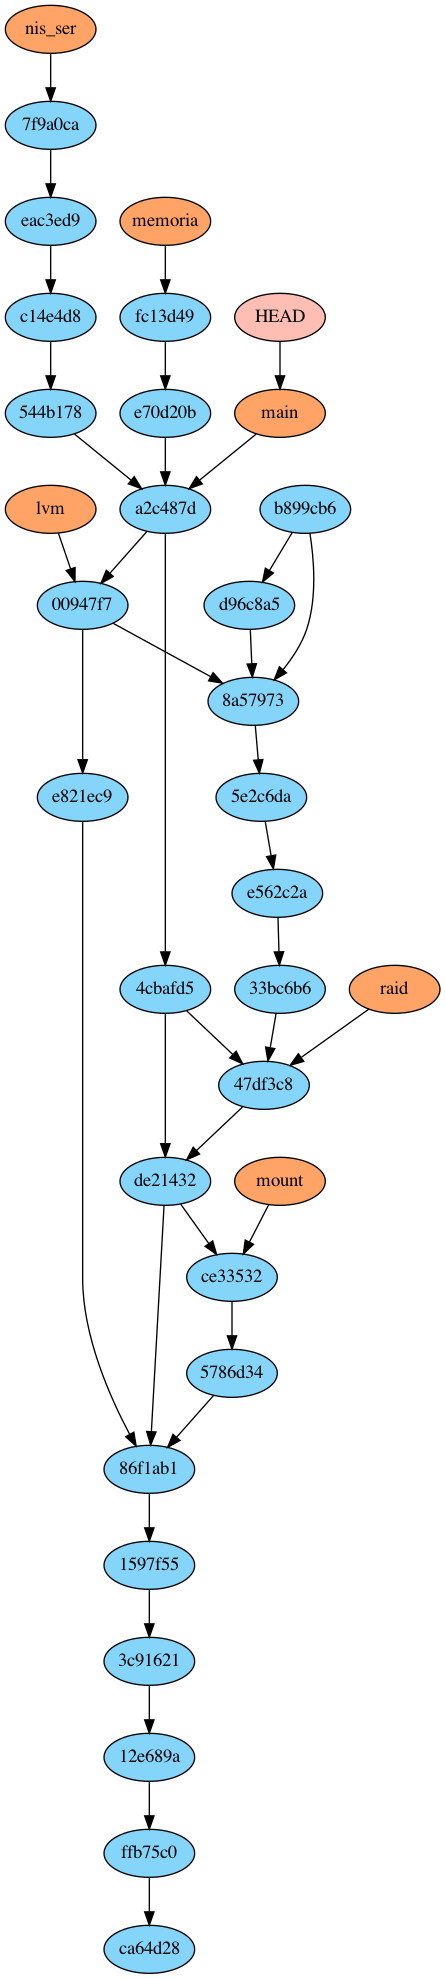
\includegraphics[trim={0 30cm 0 0}, clip, width=0.4\textwidth]{includes/graph.png}

    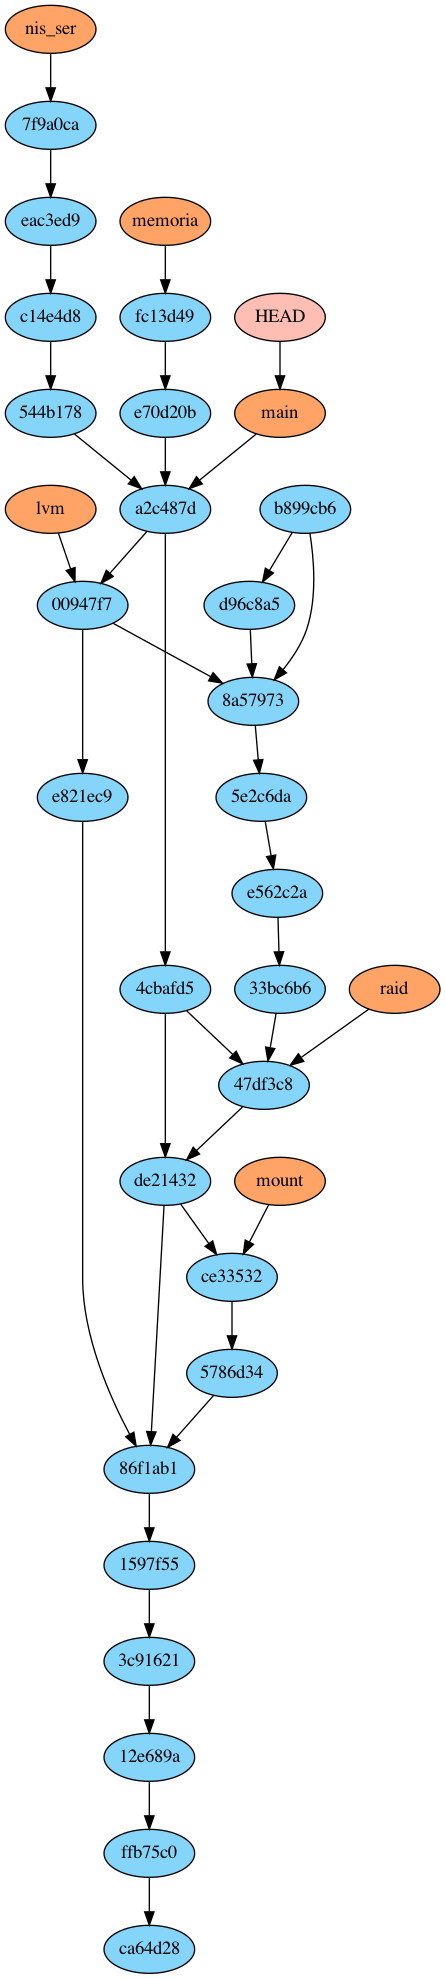
\includegraphics[trim={0 0 0 30cm}, clip, width=0.4\textwidth]{includes/graph.png}
\end{multicols}
\end{document}